\chapter{Microcontrollers}
\label{cha:microcontrollers}

C is niet beperkt tot het schrijven van programma's op de bekende besturingsystemen (Windows, Linux, mac-OSX) zoals we hebben gezien in de vorige hoofdstukken. We kunnen (en moeten) C ook gebruiken voor het schrijven van programma's op microcontrollers.

%Een \textsl{microcontroller}\index{microcontroller} is een afkorting van microprocessor\index{microprocessor} en controller. Een microprocessor is het hart van elke computer en kan met behulp van RAM, ROM en externe opslag (HDD, SSD, USB-stick) een programma uitvoeren. Zo'n microprocessor is te vinden in elke gangbare computer, voorzien van een \textsl{besturingssysteem}\index{besturingssyteem} (Engels: operaring system) zoals Windows, Linux of mac-OSX. Het besturingssysteem zorgt voor een ordentelijk verloop van de computer en de programma's. Programma's kunnen worden gestart en afgesloten, via een een grafische interface. Iedereen heeft wel eens te maken gehad met zo'n computer.

Een \textsl{microcontroller}\index{microcontroller} is een klein computersysteem waarop een microprocessor, RAM en ROM zijn ge\"integreerd. Op een microcontroller is geen besturingssysteem ge\"installeerd. We spreken dan van een \textsl{bare metal system}\index{bare metal system}. Daarnaast heeft de microcontroller \textsl{peripherals} om invoer en uitvoer naar de omgeving mogelijk te maken. Microcontrollers worden gebruikt bij eenvoudige systemen waarbij de taak van het systeem vastligt, zoals thermostaten, wasmachines en magnetrons. Invoer en uitvoer gaat niet via toetsenbord en scherm, maar via \textsl{pinnen} op de microcontroller. Een bekend systeem is de Arduino Uno met daarop een ATmega328-microcontroller. Dit systeem is te zien in figuur~\ref{fig:arduinouno}.

\begin{figure}[!ht]
\centering
\begin{tikzpicture}
\node at (0,0) {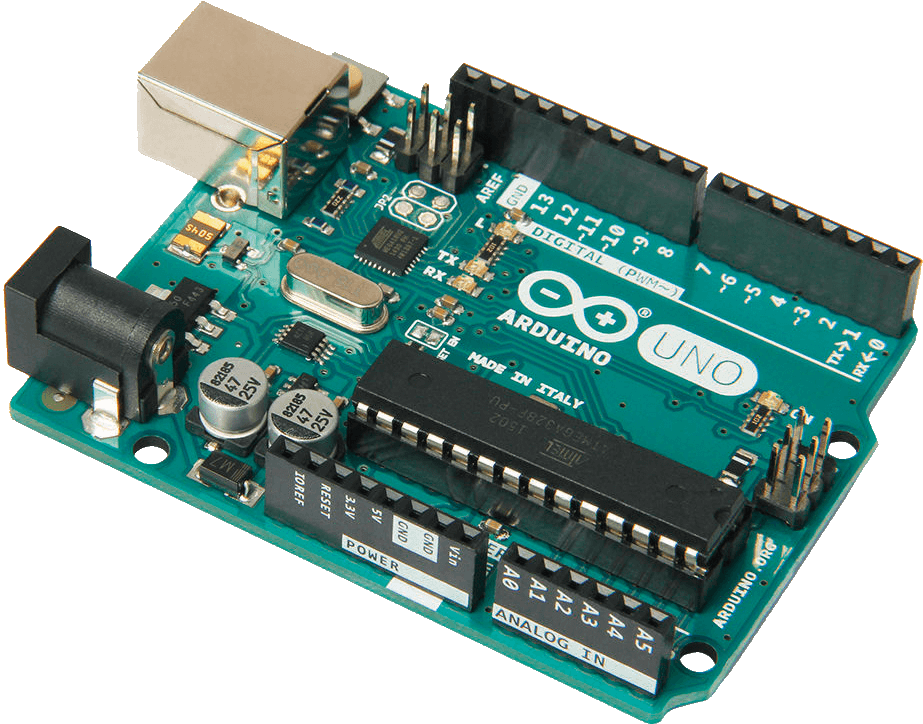
\includegraphics[scale=0.25]{images/arduino-uno-r3}};
\draw[red,*-] (0.5,-0.5) -- ++(3,0) node[right] {microcontroller};
\draw[red,*-] (-1.5,1.9) -- ++(0,.5) -- ++(2,0) node[right] {USB-connector};
\draw[red,*-] (1.5,1.3) -- ++(2,0) node[right] {headers};
\draw[red,*-] (0.0,-1.3) -- ++(3,0) node[right] {headers};
\end{tikzpicture}
\caption{Foto van een Arduino Uno met daarop een ATmega328-controller.}
\label{fig:arduinouno}
\end{figure}

Op de PCB \textsl(printed circuit board)\index{printed circuit board}\index{PCB!\see{printed circuit board}} is de microcontroller te zien (het lange, rechthoekige object). Dit is het hart van het systeem. Linksboven is een USB-connector te zien waarmee we de microcontroller kunnen programmeren en van spanning kunnen voorzien. Aan de boven- en onderkant zijn \textsl{headers}\index{headers} te zien waar we verbindingen kunnen maken met externe componenten, zoals drukknoppen en leds.

Met behulp van een programma op de PC (in dit geval de Arduino IDE, zie~\cite{arduino}), kunnen we een programma schrijven, compileren op de PC, en laden in de microcontroller. We noemen zo'n compiler een \textsl{cross compiler}\index{cross compiler} omdat we het programma niet op de PC draait maar op de microcontroller. In tegenstelling tot de gebruikelijke C-broncode, gebruikt de Arduino Uno twee specifieke functies, namelijk \lstinline|setup| en \lstinline|loop|. De functie \lstinline|setup| wordt eenmalig uitgevoerd als het programma start, de functie \lstinline|loop| wordt continu uitgevoerd zolang het programma draait. Zie listing~ \ref{cod:uno}.

\begin{lstlisting}[caption=Uitvoering op een Adruino Uno.,label=cod:uno]
void setup()
{
    /* eenmalige initialisatie */
}

void loop()
{
    /* continu uitvoeren */
}
\end{lstlisting}

We kunnen de Arduino iets zinnigs laten doen, zoals het inlezen van de stand van een pin (schakelaar) en het resultaat laten uitvoeren naar een pin (led). Dit is te zien in listing~ \ref{cod:arduinoio}. We beginnen met het defini\"eren van een aantal \textsl{pinnen}. Zie hiervoor de Arduino documentatie. Pin~7 is de input pin. Pin~13 is de output pin. De toekenningen zijn te zien in de regels~1 en~2. De variabele \lstinline|val| is een tijdelijke variabele en wordt gebruikt om de stand in te lezen en weg te schrijven.

\begin{lstlisting}[caption={Inlezen van een pin en het resultaat schrijven naar een pin.},label=cod:arduinoio]
int inPin = 7;    /* pushbutton connected to digital pin 7 */
int ledPin = 13;  /* LED connected to digital pin 13 */
int val = 0;      /* variable to store the read value */

void setup() {
  pinMode(inPin, INPUT);    /* sets the digital pin 7 as input */
  pinMode(ledPin, OUTPUT);  /* sets the digitalpin 13 as output */
}

void loop() {
  val = digitalRead(inPin);   /* read the input pin */
  digitalWrite(ledPin, val);  /* sets the LED to the button's value */
}
\end{lstlisting}

In de functie \lstinline|setup| wordt pin 7 als input bestempeld en pin~13 als output. Daarmee leggen we vast welke \textsl{richting} de pin heeft. In de functie \lstinline|loop|, die zoals eerder is vermeld continu wordt uitgevoerd, lezen we de stand van pin~7 in en schrijven dat naar pin~13. We moeten wel een schakelaar aan pin~7 en een leed aan pin~13 plaatsen, die zijn niet op het Arduino-bord aanwezig.

We kunnen ip  de PC dit programma compileren en vervolgens in de microcontroller plaatsen waarna het wordt uitgevoerd zolang de spanning aanwezig is,

Overigens zijn de functies \lstinline|setup| en \lstinline|loop| als volgt te simuleren op een PC:

\begin{lstlisting}[caption=Simulatie van de functies \texttt{setup} en \texttt{loop}.]

int main(void)
{
    setup();

    while (1)
    {
        loop();
    }
}
\end{lstlisting}

De functie \lstinline|main| is te zien als functie die aangeroepen wordt door het systeem. Daarna wordt in regel 4 eenmalig de functie \lstinline|setup| aangeroepen. De functie \lstinline|loop| wordt herhaaldelijk aangeroepen in de functie \lstinline|main|.